\documentclass{ximera}

%\usepackage{todonotes}

\newcommand{\todo}{}

\usepackage{esint} % for \oiint
\ifxake%%https://math.meta.stackexchange.com/questions/9973/how-do-you-render-a-closed-surface-double-integral
\renewcommand{\oiint}{{\large\bigcirc}\kern-1.56em\iint}
\fi


\graphicspath{
  {./}
  {ximeraTutorial/}
  {basicPhilosophy/}
  {functionsOfSeveralVariables/}
  {normalVectors/}
  {lagrangeMultipliers/}
  {vectorFields/}
  {greensTheorem/}
  {shapeOfThingsToCome/}
  {dotProducts/}
  {partialDerivativesAndTheGradientVector/}
  {../productAndQuotientRules/exercises/}
  {../normalVectors/exercisesParametricPlots/}
  {../continuityOfFunctionsOfSeveralVariables/exercises/}
  {../partialDerivativesAndTheGradientVector/exercises/}
  {../directionalDerivativeAndChainRule/exercises/}
  {../commonCoordinates/exercisesCylindricalCoordinates/}
  {../commonCoordinates/exercisesSphericalCoordinates/}
  {../greensTheorem/exercisesCurlAndLineIntegrals/}
  {../greensTheorem/exercisesDivergenceAndLineIntegrals/}
  {../shapeOfThingsToCome/exercisesDivergenceTheorem/}
  {../greensTheorem/}
  {../shapeOfThingsToCome/}
  {../separableDifferentialEquations/exercises/}
  {vectorFields/}
}

\newcommand{\mooculus}{\textsf{\textbf{MOOC}\textnormal{\textsf{ULUS}}}}

\usepackage{tkz-euclide}
\usepackage{tikz}
\usepackage{tikz-cd}
\usetikzlibrary{arrows}
\tikzset{>=stealth,commutative diagrams/.cd,
  arrow style=tikz,diagrams={>=stealth}} %% cool arrow head
\tikzset{shorten <>/.style={ shorten >=#1, shorten <=#1 } } %% allows shorter vectors

\usetikzlibrary{backgrounds} %% for boxes around graphs
\usetikzlibrary{shapes,positioning}  %% Clouds and stars
\usetikzlibrary{matrix} %% for matrix
\usepgfplotslibrary{polar} %% for polar plots
\usepgfplotslibrary{fillbetween} %% to shade area between curves in TikZ
%\usetkzobj{all}
\usepackage[makeroom]{cancel} %% for strike outs
%\usepackage{mathtools} %% for pretty underbrace % Breaks Ximera
%\usepackage{multicol}
\usepackage{pgffor} %% required for integral for loops



%% http://tex.stackexchange.com/questions/66490/drawing-a-tikz-arc-specifying-the-center
%% Draws beach ball
\tikzset{pics/carc/.style args={#1:#2:#3}{code={\draw[pic actions] (#1:#3) arc(#1:#2:#3);}}}



\usepackage{array}
\setlength{\extrarowheight}{+.1cm}
\newdimen\digitwidth
\settowidth\digitwidth{9}
\def\divrule#1#2{
\noalign{\moveright#1\digitwidth
\vbox{\hrule width#2\digitwidth}}}




% \newcommand{\RR}{\mathbb R}
% \newcommand{\R}{\mathbb R}
% \newcommand{\N}{\mathbb N}
% \newcommand{\Z}{\mathbb Z}

\newcommand{\sagemath}{\textsf{SageMath}}


%\renewcommand{\d}{\,d\!}
%\renewcommand{\d}{\mathop{}\!d}
%\newcommand{\dd}[2][]{\frac{\d #1}{\d #2}}
%\newcommand{\pp}[2][]{\frac{\partial #1}{\partial #2}}
% \renewcommand{\l}{\ell}
%\newcommand{\ddx}{\frac{d}{\d x}}

% \newcommand{\zeroOverZero}{\ensuremath{\boldsymbol{\tfrac{0}{0}}}}
%\newcommand{\inftyOverInfty}{\ensuremath{\boldsymbol{\tfrac{\infty}{\infty}}}}
%\newcommand{\zeroOverInfty}{\ensuremath{\boldsymbol{\tfrac{0}{\infty}}}}
%\newcommand{\zeroTimesInfty}{\ensuremath{\small\boldsymbol{0\cdot \infty}}}
%\newcommand{\inftyMinusInfty}{\ensuremath{\small\boldsymbol{\infty - \infty}}}
%\newcommand{\oneToInfty}{\ensuremath{\boldsymbol{1^\infty}}}
%\newcommand{\zeroToZero}{\ensuremath{\boldsymbol{0^0}}}
%\newcommand{\inftyToZero}{\ensuremath{\boldsymbol{\infty^0}}}



% \newcommand{\numOverZero}{\ensuremath{\boldsymbol{\tfrac{\#}{0}}}}
% \newcommand{\dfn}{\textbf}
% \newcommand{\unit}{\,\mathrm}
% \newcommand{\unit}{\mathop{}\!\mathrm}
% \newcommand{\eval}[1]{\bigg[ #1 \bigg]}
% \newcommand{\seq}[1]{\left( #1 \right)}
% \renewcommand{\epsilon}{\varepsilon}
% \renewcommand{\phi}{\varphi}


% \renewcommand{\iff}{\Leftrightarrow}

% \DeclareMathOperator{\arccot}{arccot}
% \DeclareMathOperator{\arcsec}{arcsec}
% \DeclareMathOperator{\arccsc}{arccsc}
% \DeclareMathOperator{\si}{Si}
% \DeclareMathOperator{\scal}{scal}
% \DeclareMathOperator{\sign}{sign}


%% \newcommand{\tightoverset}[2]{% for arrow vec
%%   \mathop{#2}\limits^{\vbox to -.5ex{\kern-0.75ex\hbox{$#1$}\vss}}}
% \newcommand{\arrowvec}[1]{{\overset{\rightharpoonup}{#1}}}
% \renewcommand{\vec}[1]{\arrowvec{\mathbf{#1}}}
% \renewcommand{\vec}[1]{{\overset{\boldsymbol{\rightharpoonup}}{\mathbf{#1}}}}

% \newcommand{\point}[1]{\left(#1\right)} %this allows \vector{ to be changed to \vector{ with a quick find and replace
% \newcommand{\pt}[1]{\mathbf{#1}} %this allows \vec{ to be changed to \vec{ with a quick find and replace
% \newcommand{\Lim}[2]{\lim_{\point{#1} \to \point{#2}}} %Bart, I changed this to point since I want to use it.  It runs through both of the exercise and exerciseE files in limits section, which is why it was in each document to start with.

% \DeclareMathOperator{\proj}{\mathbf{proj}}
% \newcommand{\veci}{{\boldsymbol{\hat{\imath}}}}
% \newcommand{\vecj}{{\boldsymbol{\hat{\jmath}}}}
% \newcommand{\veck}{{\boldsymbol{\hat{k}}}}
% \newcommand{\vecl}{\vec{\boldsymbol{\l}}}
% \newcommand{\uvec}[1]{\mathbf{\hat{#1}}}
% \newcommand{\utan}{\mathbf{\hat{t}}}
% \newcommand{\unormal}{\mathbf{\hat{n}}}
% \newcommand{\ubinormal}{\mathbf{\hat{b}}}

% \newcommand{\dotp}{\bullet}
% \newcommand{\cross}{\boldsymbol\times}
% \newcommand{\grad}{\boldsymbol\nabla}
% \newcommand{\divergence}{\grad\dotp}
% \newcommand{\curl}{\grad\cross}
%\DeclareMathOperator{\divergence}{divergence}
%\DeclareMathOperator{\curl}[1]{\grad\cross #1}
% \newcommand{\lto}{\mathop{\longrightarrow\,}\limits}

% \renewcommand{\bar}{\overline}

\colorlet{textColor}{black}
\colorlet{background}{white}
\colorlet{penColor}{blue!50!black} % Color of a curve in a plot
\colorlet{penColor2}{red!50!black}% Color of a curve in a plot
\colorlet{penColor3}{red!50!blue} % Color of a curve in a plot
\colorlet{penColor4}{green!50!black} % Color of a curve in a plot
\colorlet{penColor5}{orange!80!black} % Color of a curve in a plot
\colorlet{penColor6}{yellow!70!black} % Color of a curve in a plot
\colorlet{fill1}{penColor!20} % Color of fill in a plot
\colorlet{fill2}{penColor2!20} % Color of fill in a plot
\colorlet{fillp}{fill1} % Color of positive area
\colorlet{filln}{penColor2!20} % Color of negative area
\colorlet{fill3}{penColor3!20} % Fill
\colorlet{fill4}{penColor4!20} % Fill
\colorlet{fill5}{penColor5!20} % Fill
\colorlet{gridColor}{gray!50} % Color of grid in a plot

\newcommand{\surfaceColor}{violet}
\newcommand{\surfaceColorTwo}{redyellow}
\newcommand{\sliceColor}{greenyellow}




\pgfmathdeclarefunction{gauss}{2}{% gives gaussian
  \pgfmathparse{1/(#2*sqrt(2*pi))*exp(-((x-#1)^2)/(2*#2^2))}%
}


%%%%%%%%%%%%%
%% Vectors
%%%%%%%%%%%%%

%% Simple horiz vectors
\renewcommand{\vector}[1]{\left\langle #1\right\rangle}


%% %% Complex Horiz Vectors with angle brackets
%% \makeatletter
%% \renewcommand{\vector}[2][ , ]{\left\langle%
%%   \def\nextitem{\def\nextitem{#1}}%
%%   \@for \el:=#2\do{\nextitem\el}\right\rangle%
%% }
%% \makeatother

%% %% Vertical Vectors
%% \def\vector#1{\begin{bmatrix}\vecListA#1,,\end{bmatrix}}
%% \def\vecListA#1,{\if,#1,\else #1\cr \expandafter \vecListA \fi}

%%%%%%%%%%%%%
%% End of vectors
%%%%%%%%%%%%%

%\newcommand{\fullwidth}{}
%\newcommand{\normalwidth}{}



%% makes a snazzy t-chart for evaluating functions
%\newenvironment{tchart}{\rowcolors{2}{}{background!90!textColor}\array}{\endarray}

%%This is to help with formatting on future title pages.
\newenvironment{sectionOutcomes}{}{}



%% Flowchart stuff
%\tikzstyle{startstop} = [rectangle, rounded corners, minimum width=3cm, minimum height=1cm,text centered, draw=black]
%\tikzstyle{question} = [rectangle, minimum width=3cm, minimum height=1cm, text centered, draw=black]
%\tikzstyle{decision} = [trapezium, trapezium left angle=70, trapezium right angle=110, minimum width=3cm, minimum height=1cm, text centered, draw=black]
%\tikzstyle{question} = [rectangle, rounded corners, minimum width=3cm, minimum height=1cm,text centered, draw=black]
%\tikzstyle{process} = [rectangle, minimum width=3cm, minimum height=1cm, text centered, draw=black]
%\tikzstyle{decision} = [trapezium, trapezium left angle=70, trapezium right angle=110, minimum width=3cm, minimum height=1cm, text centered, draw=black]


\title{Quadratic Forms}

\begin{document}

\begin{abstract}
complete the square
\end{abstract}
\maketitle



We have seen that the trajectories of projectiles are described by quadratic equations.  In fact, quadratic equations and formulas are used everywhere.


\begin{itemize}
\item \link[101 Uses of a Quadratic Equation Part 1]{https://plus.maths.org/content/101-uses-quadratic-equation}
\item \link[101 Uses of a Quadratic Equation Part 2]{https://plus.maths.org/content/101-uses-quadratic-equation-part-ii}
\end{itemize}







\subsection*{Quadratic Functions}


\begin{definition} \textbf{\textcolor{green!50!black}{Quadratic Functions}} \\
\textbf{Quadratic functions} are functions which can be described with a formula of the form

\[  Q(t) = a \, t^2 + b \, t + c  \]

where $a$, $b$, and $c$ (called \textbf{coefficients}) are real numbers with $a \ne 0$



\begin{itemize}
\item $a$ is called the \textbf{leading coefficient} 
\item $a \, t^2$ is called the \textbf{leading or quadratic term} 
\item $b \, t$ is called the \textbf{linear term} 
\item $c$ is called the \textbf{constant term} 
\end{itemize}

\end{definition}




As we have seen the graph of a quadratic equation is a parabola. The sign of the leading coefficient determines if the parabola opens up or down.





\begin{image}
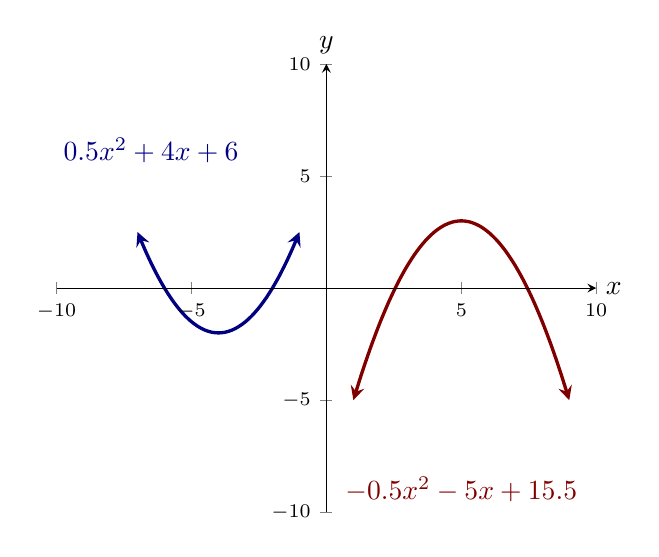
\begin{tikzpicture}
     \begin{axis}[
            	domain=-10:10, ymax=10, xmax=10, ymin=-10, xmin=-10,
            	axis lines =center, xlabel=$x$, ylabel=$y$,
               ytick={-10,-5,5,10},
               xtick={-10,-5,5,10},
               ticklabel style={font=\scriptsize},
            	every axis y label/.style={at=(current axis.above origin),anchor=south},
            	every axis x label/.style={at=(current axis.right of origin),anchor=west},
            	axis on top,
          		]


        \addplot [draw=penColor, very thick, smooth, domain=(-7:-1),<->] {0.5*(x+4)^2 -2};
        \addplot [draw=penColor2, very thick, smooth, domain=(1:9),<->] {-0.5*(x-5)^2 +3};

        

		\node[penColor] at (axis cs:-6.5,6.125) {$0.5 x^2 + 4 x + 6$};
		\node[penColor2] at (axis cs:5,-9) {$-0.5 x^2 - 5 x + 15.5$};



    \end{axis}
\end{tikzpicture}
\end{image}


\subsection*{Quadratic Function Analysis}

What do we want to know when we analyze any function?

We want to know the 
\begin{itemize}
     \item \textbf{\textcolor{red!80!black}{Domain}} 
     \item \textbf{\textcolor{red!80!black}{Zeros}} 
     \item \textbf{\textcolor{red!80!black}{Continuity}} 
\begin{itemize}
     \item \textbf{\textcolor{purple!85!blue}{discontinuities}} 
     \item \textbf{\textcolor{purple!85!blue}{singularities}} 
\end{itemize}
     \item \textbf{\textcolor{red!80!black}{End-Behavior}} 
     \item \textbf{\textcolor{red!80!black}{Behavior}} 
\begin{itemize}
     \item \textbf{\textcolor{purple!85!blue}{intervals where increasing}} 
     \item \textbf{\textcolor{purple!85!blue}{intervals where decreasing}} 
\end{itemize}
     \item \textbf{\textcolor{red!80!black}{Global Maximum and Minimum}} 
     \item \textbf{\textcolor{red!80!black}{Local Maximums and Minimums}} 
     \item \textbf{\textcolor{red!80!black}{Range}} 
     \item \textbf{\textcolor{blue!55!black}{...and we would like a nice graph}} 
\end{itemize}



\textbf{\textcolor{blue!75!black}{Quadratic Domain and Range}} \\


The implied or natural domain of a quadratic function is all real numbers.  Of course, any quadratic function could come with a stated domain that restricts the domain. Or, a quadratic might be a piece of a piecewise defined function and only applied to a stated subset of the whole domain. Or, the quadratic function might be used as a model and the situation restricts the domain to an applied domain. \\


From the graphs above we can see that the natural range of a quadratic comes in two types.  

\begin{itemize}
\item The range could be all real numbers greater than or equal to some particular real number (the minimum).
\item The range could be all real numbers less than or equal to some particular real number (the maximum).
\end{itemize}

If there is a stated domain, then the range will be restricted accordingly. \\





\textbf{\textcolor{blue!75!black}{Quadratic Zeros}} \\

The number $0$ has a unique property appropriately named as the \textbf{Zero Product Property}.  



\begin{definition}  \textbf{\textcolor{green!50!black}{Zero Product Property}} \\

If $a$ and $b$ are real numbers and $a\cdot b = 0$, then either $a=0$ or $b=0$.

\end{definition}


Zero is the ONLY number with such an identifiable test, therefore, we use it...\textbf{\textcolor{purple!85!blue}{A LOT}}!   Like when solving equations. \\


\begin{procedure}  \textbf{\textcolor{blue!55!black}{Solving Equations}}

We have two methods for solving equations.

\begin{itemize}
     \item If you know what to do, then go do it. \\
     \item If you do not know what to do, then get everything to one side with $0$ on the other side and factor.
\end{itemize}


Unless we happen to know something special (which we often do), when solving equations our general approach is to set everything equal to zero and then convert the expression into a product.  This process is called \textbf{factoring}.  The whole idea is to make our situation look like the \textbf{zero product property}.

\end{procedure}






We have already seen that factors correspond to zeros of our function. Thus, it comes as no surprise that identifying zeros of functions is a top priority.  Factoring is a top priority. Spotting horizontal intercepts in the graph is a top priority.

As we can see from their parabolic graphs below, quadratics can have $0$, $1$, or $2$ real zeros.  How do we find them? Factoring is one way.  







\begin{image}
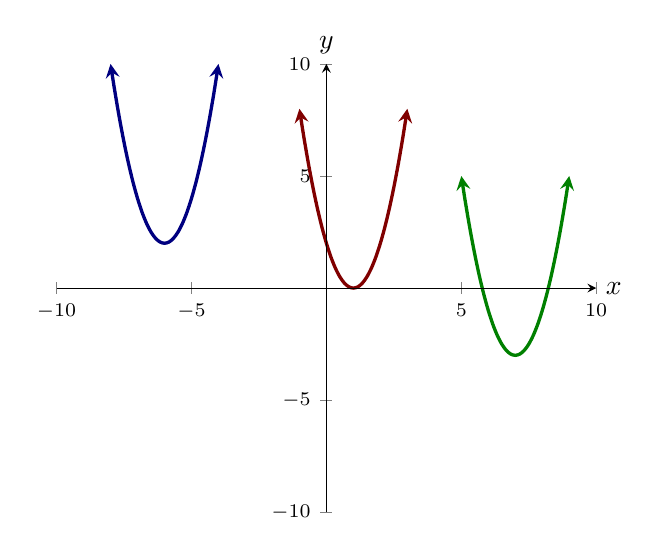
\begin{tikzpicture}
     \begin{axis}[
            	domain=-10:10, ymax=10, xmax=10, ymin=-10, xmin=-10,
            	axis lines =center, xlabel=$x$, ylabel=$y$,
               ytick={-10,-5,5,10},
               xtick={-10,-5,5,10},
               ticklabel style={font=\scriptsize},
            	every axis y label/.style={at=(current axis.above origin),anchor=south},
            	every axis x label/.style={at=(current axis.right of origin),anchor=west},
            	axis on top,
          		]


        \addplot [draw=penColor, very thick, smooth, domain=(-8:-4),<->] {2*(x+6)^2 + 2};
        \addplot [draw=penColor2, very thick, smooth, domain=(-1:3),<->] {2*(x-1)^2 };
        \addplot [draw=penColor4, very thick, smooth, domain=(5:9),<->] {2*(x-7)^2 - 3};
        

		%\node[penColor] at (axis cs:-6.5,6.125) {$0.5 x^2 + 4 x + 6$};
		%\node[penColor] at (axis cs:5,-9) {$-0.5 x^2 - 5 x + 15.5$};



    \end{axis}
\end{tikzpicture}
\end{image}





\begin{example}

Let $Q(x) = 3 \, x^2 - 5 \, x - 2$ be quadratic function. \\

What are its zeros? \\

We currently have $Q$ written in standard form, which is a sum.  We would prefer $Q$ written as a product so that we can use the zero Product Property.  This means factoring. \\


\[
Q(x) = (3 \, x + 1)(x - 2)
\]

Now, we want to know when this equals $0$. \\


$Q(x) = (3 \, x + 1)(x - 2) =0$ \\

By the zero product property, either $3 \, x + 1 = 0$ or $x - 2 = 0$. \\

This tells us that $-\frac{1}{3}$ and $2$ are zeros of $Q$.




\end{example}



Factoring is nice, provided you can think up the factors.  Sometimes, the factors are not so easy to imagine. \\


So far, we have seen the standard and factored forms for quadratics. We have a third form called the vertex form and we can convert our formula for $Q$ in this form by \textbf{completing the square}.





\subsection*{Completing the Square}

Completing the square is an algebraic procedure.  Later in this section, we will take a functional viewpoint of this (which will be more direct than the procedure below). \\



Zeros of linear functions were easy to identify.  Simply apply a little algebra to the equation to get the variable by itself on one side of the equation.  But, this is not always possible with equations of the form $0 = a \, t^2 + b \, t + c $, because there are two occurrences of the variable and they have different degrees. \\


It will take a bit of Algebra to combine them into just one occurrence. This procedure is called \textbf{completing the square}. \\



\begin{idea}


The idea is to rearrange  $0 = a \, t^2 + b \, t + c$ to look like $0 = A \, (t-B)^2 + C$.  Then there will only be  one occurrence of the $t$ and we can solve for it.


To accomplish this, we need to investigate $A \, (t-B)^2 + C$. For the moment, let's multiply it back out.


\begin{align*}
A \, (t-B)^2 + C & = A \, (t-B)(t-B) + C \\
& = A \, (t^2 - \answer{2 t B} + B^2) + C  \\
& = A \, t^2 - \answer{2 t A B} + A \, B^2 + C
\end{align*}

This last line, $A \, t^2 - 2 t A B + A \, B^2 + C$ should turn out to be $a \, t^2 + b \, t + c$, our original quadratic.

\end{idea}






We want


\[ A \, t^2 - 2 t A B + A \, B^2 + C = a \, t^2 + b \, t + c \]



The only way that is going to happen is if $A = a$. And, as long as we know $A = a$, we can factor it out and work with what is left.

Then, let's pretend our first step is factoring out $A$ or $a$ and let's start over. \\






\textbf{\textcolor{blue!75!black}{Step 1}} \\

 Factor out the leading coefficent.   In this way we can pretend that we had a \textbf{monic} quadratic from the beginning.  That means we can pretend the leading coefficient was $1$.


Starting over...starting with a leading coefficient of $1$...


\textbf{\textcolor{blue!75!black}{Step 2}} \\


We want to complete the square on $t^2 + b \, t + c$.  When the leading coefficent is $1$, then we call this quadratic \textbf{monic}.



\begin{align*}
(t-B)^2 + C & = (t - B)(t - B) + C \\
& = t^2 - 2 \, t \, B + B^2 + C  
\end{align*}


This last line $t^2 - 2 \, t \, B + B^2 + C$ should turn out to be $t^2 + b \, t + c$.

We want


\[   t^2 - 2 \, t \, B + B^2 + C = t^2 + b \, t + c   \]



\begin{explanation}


The leading term is $1$ in both (since we factored out $A$). Now, the linear terms need to be the same: $ - 2 \, t \, B = \answer{b t}$.  That tells us that $B = \answer{\frac{b}{-2}}$.

\end{explanation}


To complete the square with a monic quadratic, we need $B = \frac{b}{-2} = -\frac{b}{2}$.  Let's put that in.


\[ t^2 - 2 \, t \, B + B^2 + C = t^2 - 2 t \left( -\frac{b}{2} \right) + \left( -\frac{b}{2} \right)^2 + C = t^2 + b \, t + \left(-\frac{b}{2}\right)^2 + C \]


We want this to be $t^2 + b \, t + c$. \\

leading terms match...check \\
linear terms match...check \\


\textbf{\textcolor{blue!75!black}{Step 3}} \\


Now there is a mess for the constant term.  We have $\left( -\frac{b}{2}\right )^2 + C$, when we just wanted $c$.  \\

Then let's just pick $C$ to be $-\left( -\frac{b}{2}\right )^2 + c = -\left(\frac{b}{2}\right)^2 + c$



Whew!

Let's see some examples








\begin{example} \textit{Completing the Square}



Completing the square for $2 \, t^2 + 4 \, t + 6$.


\begin{explanation}

$\blacktriangleright$ Factor out the leading coefficent, $2$.\\

\[     2 \, t^2 + 4 \, t + 6 = 2 \left( \answer{t^2 + 2 \, t + 3} \right)   \] 


Now we have a monic to work with inside the parentheses. \\


$\blacktriangleright$ Let's move inside the parentheses.

\[ t^2 + 2 \, t + 3 \]

Take half of the linear coefficient, $\frac{2}{2} = 1$, square that $1^2 = 1$, and add and subtract it, so that we have just added $0$ to the expression and not changed its value.


\[ t^2 + 2 \, t + 1 - 1 +3 \]


Now, group.

\[ (t^2 + 2 \, t + 1) - 1 + 3 \]

the grouped part is a square.

\[ \left( \answer{t+1} \right)^2 - 1 + 3 \]

\[ (t+1)^2 + 2 \]

Remember, this was inside parentheses.

\[     2 \, t^2 + 4 \, t + 6 = 2 (t^2 + 2 \, t + 3)  = 2 ((t+1)^2 + 2) =  2 (t+1)^2 + \answer{4}\] 


$2 (t+1)^2 + 4$ is the completed square form of $2 \, t^2 + 4 \, t + 6$ \\


$2 (t+1)^2 + 4 = 2 \, t^2 + 4 \, t + 6$

\end{explanation}



\end{example}














The whole point was to change from an expression with two occurences of the variable to an expression with only one occurence of the variable. \\

This makes solving for zeros much easier. \\

Instead of solving $2 \, t^2 + 4 \, t + 6 = 0$, we can solve $2 (t+1)^2 + 4 = 0$.


\[
2 (t+1)^2 + 4 = 0
\]


\[
(t+1)^2 = -2
\]


From this equation, we can see that this function has no zeros. We wouldn't have been able to guess the factors. \\


As we saw earlier, quadratic functions can have two real zeros, one real zero, or no real zeros. \\








\begin{example} \textit{Two Real Solutions}

Solve $4  t^2 - 4 \, t - 8 = 0$ \\


\begin{explanation}

First complete the square.



\[ 4 \, t^2 -  4 \, t - 8 = 0 \]

\[ \answer{4} (t^2 - t - 2) = 0 \]



Half of the linear coefficient is $\answer{-\frac{1}{2}}$. \\

The square of that is $\answer{\frac{1}{4}}$. \\

We will be adding and subtracting $\answer{\frac{1}{4}}$ inside the parentheses.




\[ 4 \, (t^2 - t + \frac{1}{4} - \frac{1}{4} - 2)  \]


\[ 4 \, \left(\left(t - \frac{1}{2}\right)^2 - \frac{1}{4} - 2\right)  \]


\[ 4 \, \left(\left(t - \frac{1}{2}\right)^2 - \frac{1}{4} - 2\right)  \]

\[ 4 \, \left( \answer{t - \frac{1}{2}} \right)^2 - 1 - 8  \]

\[ 4 \, \left(t - \frac{1}{2}\right)^2 - 9  \]


One occurrence of $t$, good. Now to get $t$ by itself.

\[ 4 \, \left(t - \frac{1}{2}\right)^2 - 9 = 0  \]

\[ 4 \, \left(t - \frac{1}{2}\right)^2 = 9  \]

\[  \left(t - \frac{1}{2}\right)^2 = \answer{\frac{9}{4}}  \]

We know something special here. The only way this can happen is if \\



either   $\answer{t - \frac{1}{2}} = \frac{3}{2}$  or  $\answer{t - \frac{1}{2}} = -\frac{3}{2}$ \\

The first choice gives us $t = 2$ and the second choice gives us $t = -1$




Let's check those solutions.

\begin{itemize}
\item $4 (2)^2 - 4 (2) - 8 = 0$ ... check
\item $4 (-1)^2 - 4 (-1) - 8 = 0$ ... check
\end{itemize}



We have already seen that a quadratic equation can have at most two solutions.  So, we must have all of the solutions.

\end{explanation}


\end{example}









\begin{example} \textit{One Real Solution}

Solve $2 \, x^2 - 12 \, x + 21 = 3$ \\

\begin{explanation}


First, get everything to one side and $0$ on the other side.



\[  2 \, x^2 - 12 \, x + \answer{18} = 0  \]

Factor out $a$, which is $2$ here.

\[  2 \left( \answer{x^2 - 6x + 9} \right) = 0  \]


Square half of $b$, $\left(\frac{-6}{2}\right) = (-3)^2 = 9$.  But, $9$ is already there.  This must already be a square.



\[  2 \left( \answer{x - 3} \right)^2 = 0  \]


Now, get $x$ by itself.

\[  2 (x - 3)^2 = 0  \]

\[  (x - 3)^2 = 0  \]


Unlike $\frac{9}{4}$ in the previous example, the only number you can square and get $0$ is $0$.

\[  x - 3 = 0  \]

\[  x = 3  \]


This equation only has one solution.


\end{explanation}
\end{example}



The graph of $y = 2 \, x^2 - 12\, x + 18$ would be a parabola touching the horizontal axis at only one point (its vertex).




\begin{idea} \textbf{\textcolor{red!80!black}{Double Root}} \\

If the vertex of the parabola is the only intercept, then the corresponding quadratic function has a double root.


\end{idea}



There is another viewpoint on the example above.  We arrived at this equation

\[  (x - 3)^2 = 0  \]

which could be viewed as 

\[  (x - 3) (x - 3) = 0  \]


If we proceed with the zero product property we would create two new equations.  One for each factor.

Either $x - 3 = 0$   or $x - 3 = 0$. \\

Either $x = 3$ or $x = 3$.  \\

$3$ is the only solution to the equation, but the equation has this solution twice. \textbf{\textcolor{red!80!black}{A double root}}.


The previous two examples illustrated that quadratic equations can have two or one solutions.  And, a quadratic equation can have no real solutions.










\begin{example} \textit{No Real Solutions}

Solve $2 \, x^2 - 12 \, x + 21 = 1$ \\

\begin{explanation}

First, get everything to one side and $0$ on the other side.



\[  2 \, x^2 - 12 \, x + 20 = 0  \]

Factor out the leading coefficient.

\[  2 \left( \answer{x^2 - 6x + 10} \right) = 0  \]


Square half of $b$, $\left(\frac{-6}{2}\right)^2 = (-3)^2$ and $(-3)^2 = 9$.  We could add and subtract $9$ or we can change the $10$ to be $9+1$.  All we are trying to do is to see a $9$.



\[  2 (x^2 - 6 \, x + 9 + 1) = 0  \]


\[  2 ((x-3)^2 + 1) = 0  \]


\[  2 (x-3)^2 + 2 = 0  \]

In the real numbers, $2 (x-3)^2$ is never negative, since we have a square.  This cannot be added to $2$, to get $0$.  \\


This equation has no real solutions.


\end{explanation}
\end{example}



The above example illustrates that there must be numbers missing from the real numbers.  We normally expect equations to have solutions. 


$\blacktriangleright$  \textbf{\textcolor{purple!85!blue}{A Peek Ahead}} 



It feels like that equation should have a solution.  


All we needed was for $(x-3)^2 = -1$ 

There are no real numebrs that will do this.  The square of a real number cannot be negative. 




We can see that the real numbers are not enough for all of our equations.  Eventually, we will fill in the missing pieces with the \textbf{Complex Numbers}.  They will include $\sqrt{-1}$.  Then our last example will have two complex solutions.  


\begin{itemize}
\item Our first example had two real solutions.  
\item Our second example had two identical solutions.  
\item This third example has two distinct complex solutions. 
\end{itemize}



$\blacktriangleright$ All quadratics will have two solutions...eventually. \\

We'll fill in the holes in the second course.









For now, we are staying inside the real numbers.



For now, we note that there are no \textbf{real} solutions in the third example.

























\begin{center}
\textbf{\textcolor{green!50!black}{ooooo-=-=-=-ooOoo-=-=-=-ooooo}} \\

more examples can be found by following this link\\ \link[More Examples of Quadratics]{https://ximera.osu.edu/csccmathematics/precalculus1/precalculus1/projectileMotion/examples/exampleList}

\end{center}











\end{document}
